% Delete D: copy successor E, delete that minimum node, then repair the red links.
% Editable source for this diagram. From this directory, regenerate with:
% latex -interaction=nonstopmode -halt-on-error llrbt-9.tex
% dvisvgm --no-fonts --exact --bbox=papersize --output=llrbt-9.svg llrbt-9.dvi
\documentclass[tikz,border=12pt]{standalone}
\usepackage{lmodern}
\usepackage{tikz}
\usetikzlibrary{arrows.meta,backgrounds,shapes.geometric,patterns}
\definecolor{linkred}{HTML}{B5240A}
\definecolor{noteBlue}{HTML}{0067A5}
\definecolor{softgreen}{HTML}{D8EAD0}
\definecolor{softpurple}{HTML}{D9D1E8}
\definecolor{softpink}{HTML}{F5CECF}
\definecolor{softyellow}{HTML}{FFF2C9}
% Translucent vector layers keep the soft shadow in the DVI-to-SVG export.
\tikzset{
  llrbt shadow layer/.style args={#1/#2}{
    preaction={fill=black,draw=none,fill opacity=#2,
      transform canvas={shift={(3pt,-3pt)},
        scale around=#1:(current path bounding box.center)}}
  },
  llrbt shadow/.style={
    llrbt shadow layer=1.40/0.01,
    llrbt shadow layer=1.35/0.015,
    llrbt shadow layer=1.30/0.025,
    llrbt shadow layer=1.25/0.04,
    llrbt shadow layer=1.20/0.06,
    llrbt shadow layer=1.15/0.08,
    llrbt shadow layer=1.10/0.10,
    llrbt shadow layer=1.05/0.12,
    llrbt shadow layer=1.00/0.14,
    llrbt shadow layer=0.95/0.16,
    llrbt shadow layer=0.90/0.18,
    llrbt shadow layer=0.85/0.20
  }
}
\begin{document}
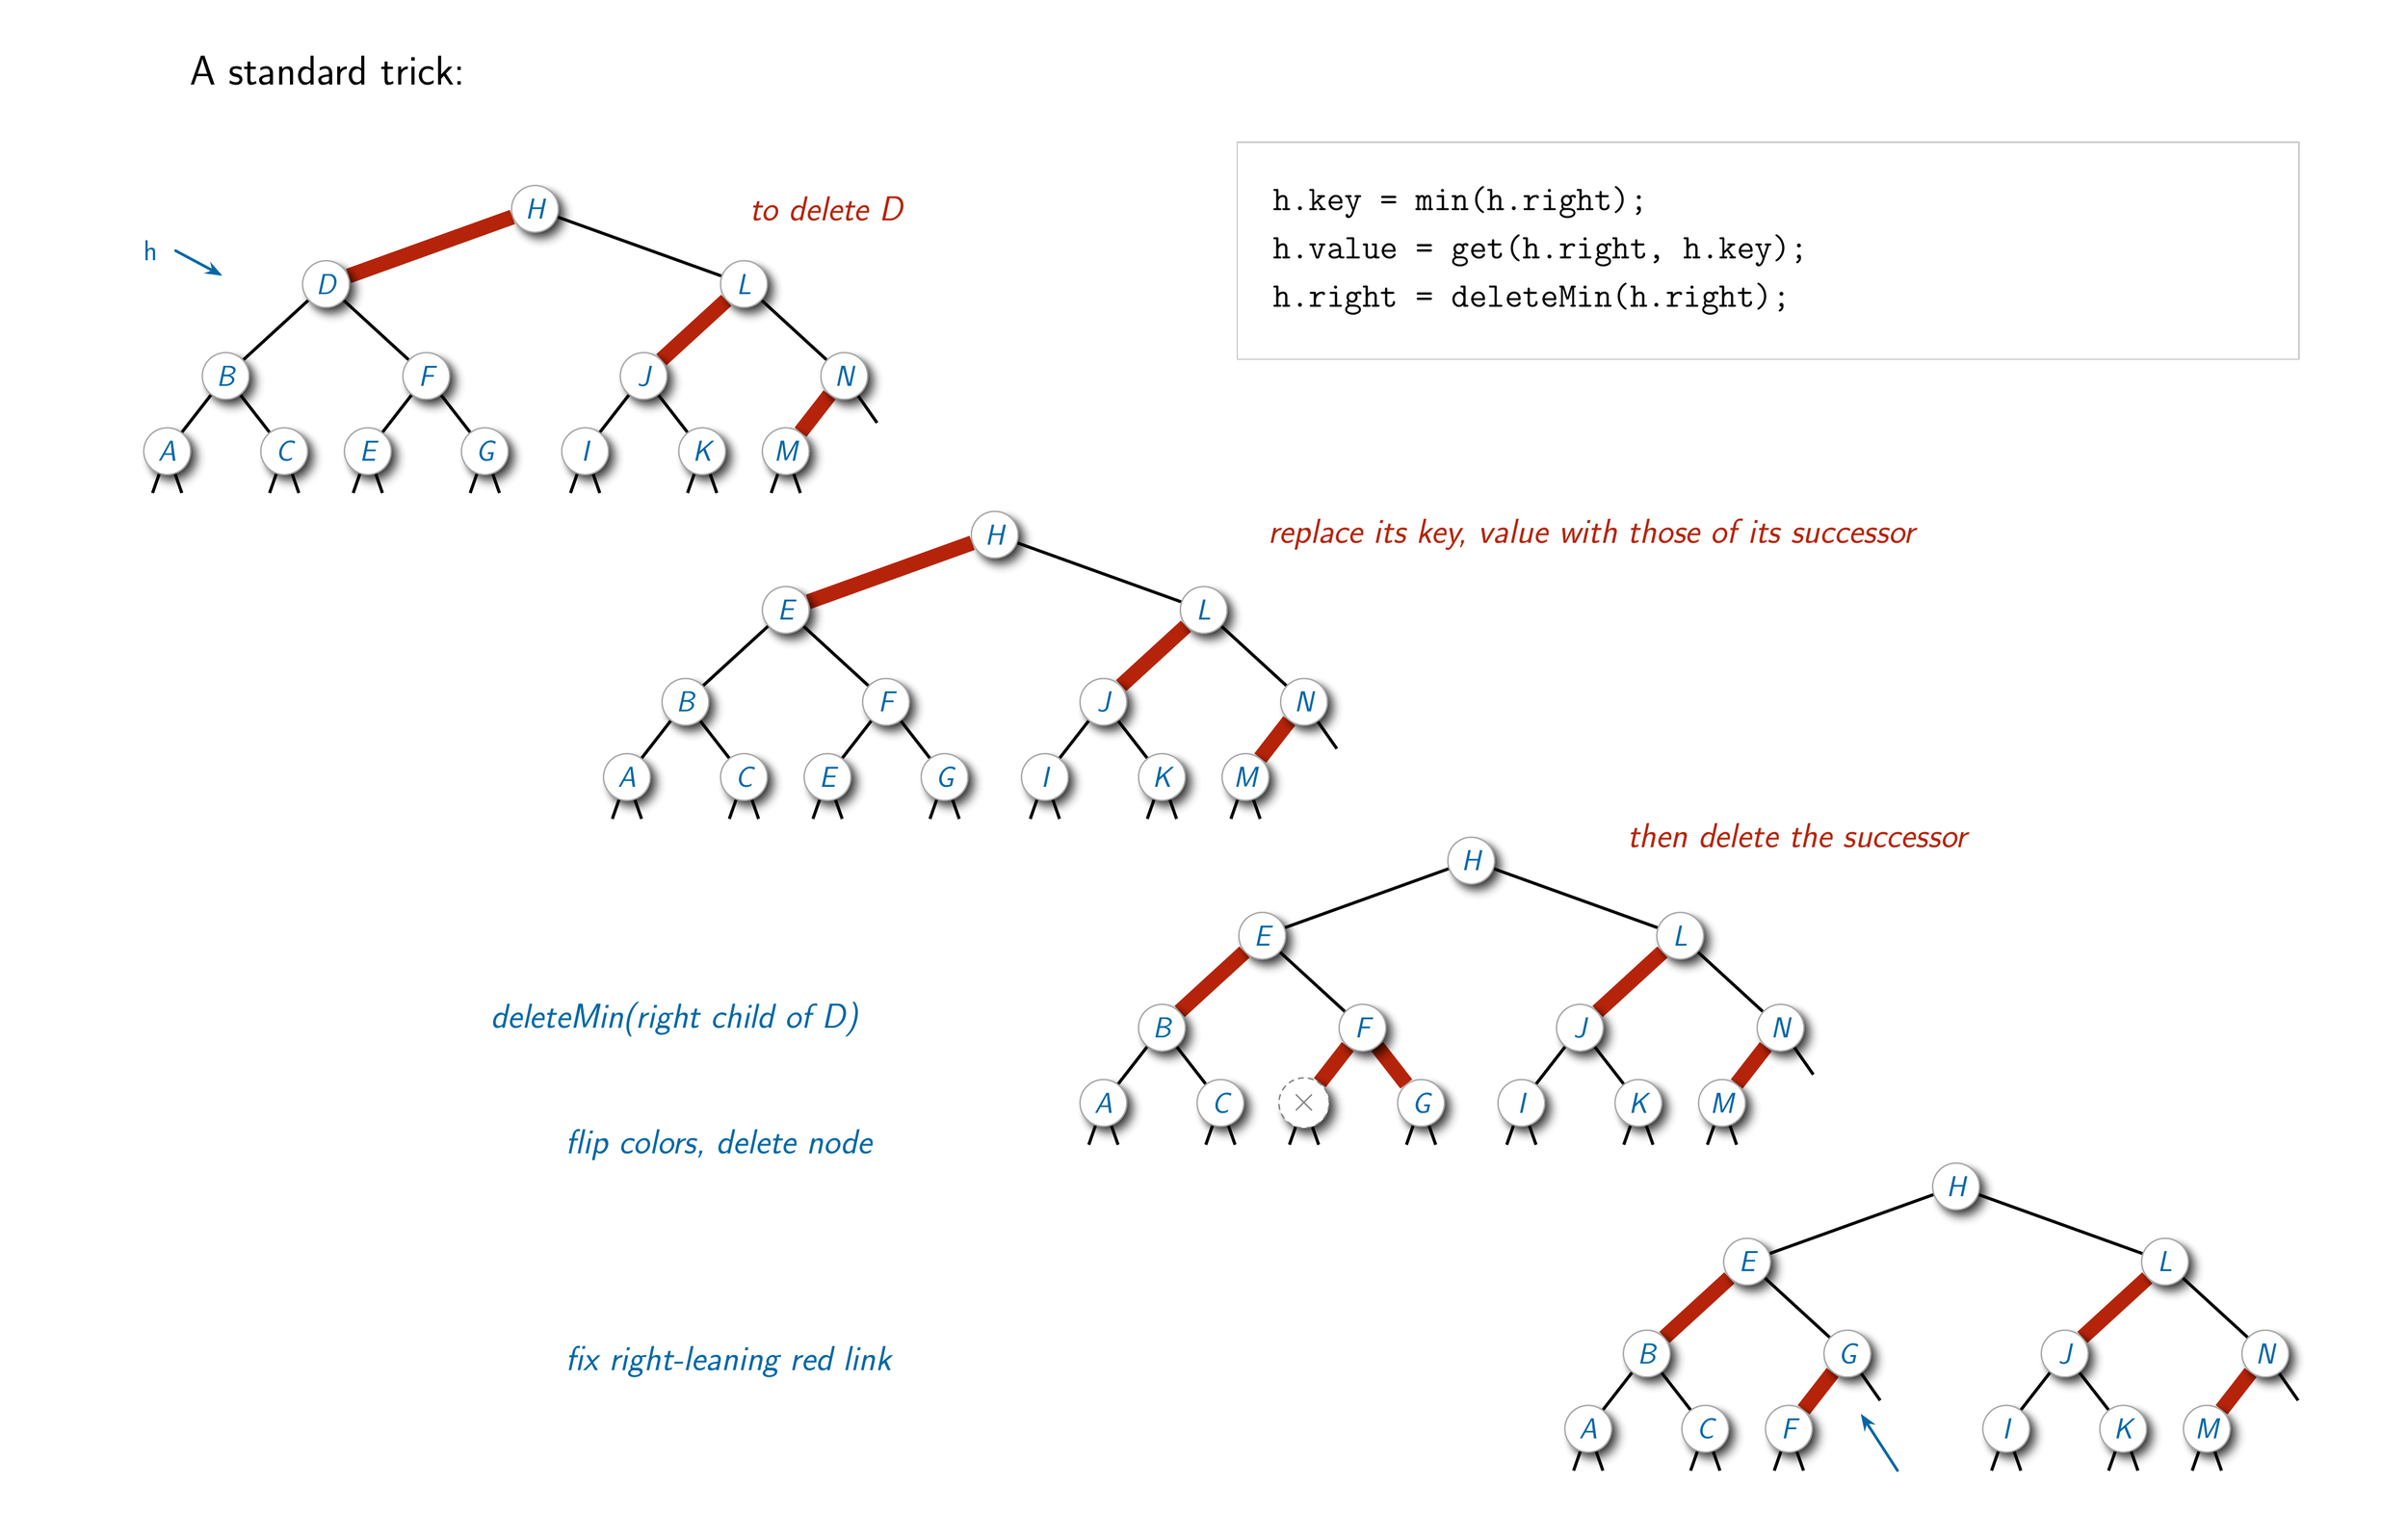
\begin{tikzpicture}[x=1pt,y=-1pt,>=Stealth,line cap=round,line join=round]
\path[use as bounding box] (0,0) rectangle (1420,900);
\begin{scope}[on background layer]
\draw[draw=black,line width=1.8pt] (90,260) -- (81.25,285);
\draw[draw=black,line width=1.8pt] (90,260) -- (98.75,285);
\draw[draw=black,line width=1.8pt] (160,260) -- (151.25,285);
\draw[draw=black,line width=1.8pt] (160,260) -- (168.75,285);
\draw[draw=black,line width=1.8pt] (210,260) -- (201.25,285);
\draw[draw=black,line width=1.8pt] (210,260) -- (218.75,285);
\draw[draw=black,line width=1.8pt] (280,260) -- (271.25,285);
\draw[draw=black,line width=1.8pt] (280,260) -- (288.75,285);
\draw[draw=black,line width=1.8pt] (340,260) -- (331.25,285);
\draw[draw=black,line width=1.8pt] (340,260) -- (348.75,285);
\draw[draw=black,line width=1.8pt] (410,260) -- (401.25,285);
\draw[draw=black,line width=1.8pt] (410,260) -- (418.75,285);
\draw[draw=black,line width=1.8pt] (460,260) -- (451.25,285);
\draw[draw=black,line width=1.8pt] (460,260) -- (468.75,285);
\draw[draw=black,line width=1.8pt] (495,215) -- (514.6,243);
\draw[draw=black,line width=1.8pt] (365,455) -- (356.25,480);
\draw[draw=black,line width=1.8pt] (365,455) -- (373.75,480);
\draw[draw=black,line width=1.8pt] (435,455) -- (426.25,480);
\draw[draw=black,line width=1.8pt] (435,455) -- (443.75,480);
\draw[draw=black,line width=1.8pt] (485,455) -- (476.25,480);
\draw[draw=black,line width=1.8pt] (485,455) -- (493.75,480);
\draw[draw=black,line width=1.8pt] (555,455) -- (546.25,480);
\draw[draw=black,line width=1.8pt] (555,455) -- (563.75,480);
\draw[draw=black,line width=1.8pt] (615,455) -- (606.25,480);
\draw[draw=black,line width=1.8pt] (615,455) -- (623.75,480);
\draw[draw=black,line width=1.8pt] (685,455) -- (676.25,480);
\draw[draw=black,line width=1.8pt] (685,455) -- (693.75,480);
\draw[draw=black,line width=1.8pt] (735,455) -- (726.25,480);
\draw[draw=black,line width=1.8pt] (735,455) -- (743.75,480);
\draw[draw=black,line width=1.8pt] (770,410) -- (789.6,438);
\draw[draw=black,line width=1.8pt] (650,650) -- (641.25,675);
\draw[draw=black,line width=1.8pt] (650,650) -- (658.75,675);
\draw[draw=black,line width=1.8pt] (720,650) -- (711.25,675);
\draw[draw=black,line width=1.8pt] (720,650) -- (728.75,675);
\draw[draw=black,line width=1.8pt] (770,650) -- (761.25,675);
\draw[draw=black,line width=1.8pt] (770,650) -- (778.75,675);
\draw[draw=black,line width=1.8pt] (840,650) -- (831.25,675);
\draw[draw=black,line width=1.8pt] (840,650) -- (848.75,675);
\draw[draw=black,line width=1.8pt] (900,650) -- (891.25,675);
\draw[draw=black,line width=1.8pt] (900,650) -- (908.75,675);
\draw[draw=black,line width=1.8pt] (970,650) -- (961.25,675);
\draw[draw=black,line width=1.8pt] (970,650) -- (978.75,675);
\draw[draw=black,line width=1.8pt] (1020,650) -- (1011.25,675);
\draw[draw=black,line width=1.8pt] (1020,650) -- (1028.75,675);
\draw[draw=black,line width=1.8pt] (1055,605) -- (1074.6,633);
\draw[draw=black,line width=1.8pt] (940,845) -- (931.25,870);
\draw[draw=black,line width=1.8pt] (940,845) -- (948.75,870);
\draw[draw=black,line width=1.8pt] (1010,845) -- (1001.25,870);
\draw[draw=black,line width=1.8pt] (1010,845) -- (1018.75,870);
\draw[draw=black,line width=1.8pt] (1190,845) -- (1181.25,870);
\draw[draw=black,line width=1.8pt] (1190,845) -- (1198.75,870);
\draw[draw=black,line width=1.8pt] (1260,845) -- (1251.25,870);
\draw[draw=black,line width=1.8pt] (1260,845) -- (1268.75,870);
\draw[draw=black,line width=1.8pt] (1310,845) -- (1301.25,870);
\draw[draw=black,line width=1.8pt] (1310,845) -- (1318.75,870);
\draw[draw=black,line width=1.8pt] (1060,845) -- (1051.25,870);
\draw[draw=black,line width=1.8pt] (1060,845) -- (1068.75,870);
\draw[draw=black,line width=1.8pt] (1345,800) -- (1364.6,828);
\draw[draw=black,line width=1.8pt] (1095,800) -- (1114.6,828);
\end{scope}
\node[llrbt shadow,circle,draw=black!35,fill=white,text=noteBlue,minimum size=28pt,inner sep=0pt,line width=0.8pt,font=\sffamily\fontsize{18}{21.6}\selectfont,font=\sffamily\itshape\fontsize{18}{22}\selectfont] (s1-H) at (310,115) {H};
\node[llrbt shadow,circle,draw=black!35,fill=white,text=noteBlue,minimum size=28pt,inner sep=0pt,line width=0.8pt,font=\sffamily\fontsize{18}{21.6}\selectfont,font=\sffamily\itshape\fontsize{18}{22}\selectfont] (s1-D) at (185,160) {D};
\node[llrbt shadow,circle,draw=black!35,fill=white,text=noteBlue,minimum size=28pt,inner sep=0pt,line width=0.8pt,font=\sffamily\fontsize{18}{21.6}\selectfont,font=\sffamily\itshape\fontsize{18}{22}\selectfont] (s1-L) at (435,160) {L};
\node[llrbt shadow,circle,draw=black!35,fill=white,text=noteBlue,minimum size=28pt,inner sep=0pt,line width=0.8pt,font=\sffamily\fontsize{18}{21.6}\selectfont,font=\sffamily\itshape\fontsize{18}{22}\selectfont] (s1-B) at (125,215) {B};
\node[llrbt shadow,circle,draw=black!35,fill=white,text=noteBlue,minimum size=28pt,inner sep=0pt,line width=0.8pt,font=\sffamily\fontsize{18}{21.6}\selectfont,font=\sffamily\itshape\fontsize{18}{22}\selectfont] (s1-F) at (245,215) {F};
\node[llrbt shadow,circle,draw=black!35,fill=white,text=noteBlue,minimum size=28pt,inner sep=0pt,line width=0.8pt,font=\sffamily\fontsize{18}{21.6}\selectfont,font=\sffamily\itshape\fontsize{18}{22}\selectfont] (s1-J) at (375,215) {J};
\node[llrbt shadow,circle,draw=black!35,fill=white,text=noteBlue,minimum size=28pt,inner sep=0pt,line width=0.8pt,font=\sffamily\fontsize{18}{21.6}\selectfont,font=\sffamily\itshape\fontsize{18}{22}\selectfont] (s1-N) at (495,215) {N};
\node[llrbt shadow,circle,draw=black!35,fill=white,text=noteBlue,minimum size=28pt,inner sep=0pt,line width=0.8pt,font=\sffamily\fontsize{18}{21.6}\selectfont,font=\sffamily\itshape\fontsize{18}{22}\selectfont] (s1-A) at (90,260) {A};
\node[llrbt shadow,circle,draw=black!35,fill=white,text=noteBlue,minimum size=28pt,inner sep=0pt,line width=0.8pt,font=\sffamily\fontsize{18}{21.6}\selectfont,font=\sffamily\itshape\fontsize{18}{22}\selectfont] (s1-C) at (160,260) {C};
\node[llrbt shadow,circle,draw=black!35,fill=white,text=noteBlue,minimum size=28pt,inner sep=0pt,line width=0.8pt,font=\sffamily\fontsize{18}{21.6}\selectfont,font=\sffamily\itshape\fontsize{18}{22}\selectfont] (s1-E) at (210,260) {E};
\node[llrbt shadow,circle,draw=black!35,fill=white,text=noteBlue,minimum size=28pt,inner sep=0pt,line width=0.8pt,font=\sffamily\fontsize{18}{21.6}\selectfont,font=\sffamily\itshape\fontsize{18}{22}\selectfont] (s1-G) at (280,260) {G};
\node[llrbt shadow,circle,draw=black!35,fill=white,text=noteBlue,minimum size=28pt,inner sep=0pt,line width=0.8pt,font=\sffamily\fontsize{18}{21.6}\selectfont,font=\sffamily\itshape\fontsize{18}{22}\selectfont] (s1-I) at (340,260) {I};
\node[llrbt shadow,circle,draw=black!35,fill=white,text=noteBlue,minimum size=28pt,inner sep=0pt,line width=0.8pt,font=\sffamily\fontsize{18}{21.6}\selectfont,font=\sffamily\itshape\fontsize{18}{22}\selectfont] (s1-K) at (410,260) {K};
\node[llrbt shadow,circle,draw=black!35,fill=white,text=noteBlue,minimum size=28pt,inner sep=0pt,line width=0.8pt,font=\sffamily\fontsize{18}{21.6}\selectfont,font=\sffamily\itshape\fontsize{18}{22}\selectfont] (s1-M) at (460,260) {M};
\node[llrbt shadow,circle,draw=black!35,fill=white,text=noteBlue,minimum size=28pt,inner sep=0pt,line width=0.8pt,font=\sffamily\fontsize{18}{21.6}\selectfont,font=\sffamily\itshape\fontsize{18}{22}\selectfont] (s2-H) at (585,310) {H};
\node[llrbt shadow,circle,draw=black!35,fill=white,text=noteBlue,minimum size=28pt,inner sep=0pt,line width=0.8pt,font=\sffamily\fontsize{18}{21.6}\selectfont,font=\sffamily\itshape\fontsize{18}{22}\selectfont] (s2-D) at (460,355) {E};
\node[llrbt shadow,circle,draw=black!35,fill=white,text=noteBlue,minimum size=28pt,inner sep=0pt,line width=0.8pt,font=\sffamily\fontsize{18}{21.6}\selectfont,font=\sffamily\itshape\fontsize{18}{22}\selectfont] (s2-L) at (710,355) {L};
\node[llrbt shadow,circle,draw=black!35,fill=white,text=noteBlue,minimum size=28pt,inner sep=0pt,line width=0.8pt,font=\sffamily\fontsize{18}{21.6}\selectfont,font=\sffamily\itshape\fontsize{18}{22}\selectfont] (s2-B) at (400,410) {B};
\node[llrbt shadow,circle,draw=black!35,fill=white,text=noteBlue,minimum size=28pt,inner sep=0pt,line width=0.8pt,font=\sffamily\fontsize{18}{21.6}\selectfont,font=\sffamily\itshape\fontsize{18}{22}\selectfont] (s2-F) at (520,410) {F};
\node[llrbt shadow,circle,draw=black!35,fill=white,text=noteBlue,minimum size=28pt,inner sep=0pt,line width=0.8pt,font=\sffamily\fontsize{18}{21.6}\selectfont,font=\sffamily\itshape\fontsize{18}{22}\selectfont] (s2-J) at (650,410) {J};
\node[llrbt shadow,circle,draw=black!35,fill=white,text=noteBlue,minimum size=28pt,inner sep=0pt,line width=0.8pt,font=\sffamily\fontsize{18}{21.6}\selectfont,font=\sffamily\itshape\fontsize{18}{22}\selectfont] (s2-N) at (770,410) {N};
\node[llrbt shadow,circle,draw=black!35,fill=white,text=noteBlue,minimum size=28pt,inner sep=0pt,line width=0.8pt,font=\sffamily\fontsize{18}{21.6}\selectfont,font=\sffamily\itshape\fontsize{18}{22}\selectfont] (s2-A) at (365,455) {A};
\node[llrbt shadow,circle,draw=black!35,fill=white,text=noteBlue,minimum size=28pt,inner sep=0pt,line width=0.8pt,font=\sffamily\fontsize{18}{21.6}\selectfont,font=\sffamily\itshape\fontsize{18}{22}\selectfont] (s2-C) at (435,455) {C};
\node[llrbt shadow,circle,draw=black!35,fill=white,text=noteBlue,minimum size=28pt,inner sep=0pt,line width=0.8pt,font=\sffamily\fontsize{18}{21.6}\selectfont,font=\sffamily\itshape\fontsize{18}{22}\selectfont] (s2-E) at (485,455) {E};
\node[llrbt shadow,circle,draw=black!35,fill=white,text=noteBlue,minimum size=28pt,inner sep=0pt,line width=0.8pt,font=\sffamily\fontsize{18}{21.6}\selectfont,font=\sffamily\itshape\fontsize{18}{22}\selectfont] (s2-G) at (555,455) {G};
\node[llrbt shadow,circle,draw=black!35,fill=white,text=noteBlue,minimum size=28pt,inner sep=0pt,line width=0.8pt,font=\sffamily\fontsize{18}{21.6}\selectfont,font=\sffamily\itshape\fontsize{18}{22}\selectfont] (s2-I) at (615,455) {I};
\node[llrbt shadow,circle,draw=black!35,fill=white,text=noteBlue,minimum size=28pt,inner sep=0pt,line width=0.8pt,font=\sffamily\fontsize{18}{21.6}\selectfont,font=\sffamily\itshape\fontsize{18}{22}\selectfont] (s2-K) at (685,455) {K};
\node[llrbt shadow,circle,draw=black!35,fill=white,text=noteBlue,minimum size=28pt,inner sep=0pt,line width=0.8pt,font=\sffamily\fontsize{18}{21.6}\selectfont,font=\sffamily\itshape\fontsize{18}{22}\selectfont] (s2-M) at (735,455) {M};
\node[llrbt shadow,circle,draw=black!35,fill=white,text=noteBlue,minimum size=28pt,inner sep=0pt,line width=0.8pt,font=\sffamily\fontsize{18}{21.6}\selectfont,font=\sffamily\itshape\fontsize{18}{22}\selectfont] (s3-H) at (870,505) {H};
\node[llrbt shadow,circle,draw=black!35,fill=white,text=noteBlue,minimum size=28pt,inner sep=0pt,line width=0.8pt,font=\sffamily\fontsize{18}{21.6}\selectfont,font=\sffamily\itshape\fontsize{18}{22}\selectfont] (s3-D) at (745,550) {E};
\node[llrbt shadow,circle,draw=black!35,fill=white,text=noteBlue,minimum size=28pt,inner sep=0pt,line width=0.8pt,font=\sffamily\fontsize{18}{21.6}\selectfont,font=\sffamily\itshape\fontsize{18}{22}\selectfont] (s3-L) at (995,550) {L};
\node[llrbt shadow,circle,draw=black!35,fill=white,text=noteBlue,minimum size=28pt,inner sep=0pt,line width=0.8pt,font=\sffamily\fontsize{18}{21.6}\selectfont,font=\sffamily\itshape\fontsize{18}{22}\selectfont] (s3-B) at (685,605) {B};
\node[llrbt shadow,circle,draw=black!35,fill=white,text=noteBlue,minimum size=28pt,inner sep=0pt,line width=0.8pt,font=\sffamily\fontsize{18}{21.6}\selectfont,font=\sffamily\itshape\fontsize{18}{22}\selectfont] (s3-F) at (805,605) {F};
\node[llrbt shadow,circle,draw=black!35,fill=white,text=noteBlue,minimum size=28pt,inner sep=0pt,line width=0.8pt,font=\sffamily\fontsize{18}{21.6}\selectfont,font=\sffamily\itshape\fontsize{18}{22}\selectfont] (s3-J) at (935,605) {J};
\node[llrbt shadow,circle,draw=black!35,fill=white,text=noteBlue,minimum size=28pt,inner sep=0pt,line width=0.8pt,font=\sffamily\fontsize{18}{21.6}\selectfont,font=\sffamily\itshape\fontsize{18}{22}\selectfont] (s3-N) at (1055,605) {N};
\node[llrbt shadow,circle,draw=black!35,fill=white,text=noteBlue,minimum size=28pt,inner sep=0pt,line width=0.8pt,font=\sffamily\fontsize{18}{21.6}\selectfont,font=\sffamily\itshape\fontsize{18}{22}\selectfont] (s3-A) at (650,650) {A};
\node[llrbt shadow,circle,draw=black!35,fill=white,text=noteBlue,minimum size=28pt,inner sep=0pt,line width=0.8pt,font=\sffamily\fontsize{18}{21.6}\selectfont,font=\sffamily\itshape\fontsize{18}{22}\selectfont] (s3-C) at (720,650) {C};
\node[llrbt shadow,circle,draw=black!50,fill=white,text=black!50,minimum size=30pt,inner sep=0pt,line width=0.8pt,font=\sffamily\fontsize{21}{25.2}\selectfont,dashed] (s3-E) at (770,650) {\(\times\)};
\node[llrbt shadow,circle,draw=black!35,fill=white,text=noteBlue,minimum size=28pt,inner sep=0pt,line width=0.8pt,font=\sffamily\fontsize{18}{21.6}\selectfont,font=\sffamily\itshape\fontsize{18}{22}\selectfont] (s3-G) at (840,650) {G};
\node[llrbt shadow,circle,draw=black!35,fill=white,text=noteBlue,minimum size=28pt,inner sep=0pt,line width=0.8pt,font=\sffamily\fontsize{18}{21.6}\selectfont,font=\sffamily\itshape\fontsize{18}{22}\selectfont] (s3-I) at (900,650) {I};
\node[llrbt shadow,circle,draw=black!35,fill=white,text=noteBlue,minimum size=28pt,inner sep=0pt,line width=0.8pt,font=\sffamily\fontsize{18}{21.6}\selectfont,font=\sffamily\itshape\fontsize{18}{22}\selectfont] (s3-K) at (970,650) {K};
\node[llrbt shadow,circle,draw=black!35,fill=white,text=noteBlue,minimum size=28pt,inner sep=0pt,line width=0.8pt,font=\sffamily\fontsize{18}{21.6}\selectfont,font=\sffamily\itshape\fontsize{18}{22}\selectfont] (s3-M) at (1020,650) {M};
\node[llrbt shadow,circle,draw=black!35,fill=white,text=noteBlue,minimum size=28pt,inner sep=0pt,line width=0.8pt,font=\sffamily\fontsize{18}{21.6}\selectfont,font=\sffamily\itshape\fontsize{18}{22}\selectfont] (s4-H) at (1160,700) {H};
\node[llrbt shadow,circle,draw=black!35,fill=white,text=noteBlue,minimum size=28pt,inner sep=0pt,line width=0.8pt,font=\sffamily\fontsize{18}{21.6}\selectfont,font=\sffamily\itshape\fontsize{18}{22}\selectfont] (s4-D) at (1035,745) {E};
\node[llrbt shadow,circle,draw=black!35,fill=white,text=noteBlue,minimum size=28pt,inner sep=0pt,line width=0.8pt,font=\sffamily\fontsize{18}{21.6}\selectfont,font=\sffamily\itshape\fontsize{18}{22}\selectfont] (s4-L) at (1285,745) {L};
\node[llrbt shadow,circle,draw=black!35,fill=white,text=noteBlue,minimum size=28pt,inner sep=0pt,line width=0.8pt,font=\sffamily\fontsize{18}{21.6}\selectfont,font=\sffamily\itshape\fontsize{18}{22}\selectfont] (s4-B) at (975,800) {B};
\node[llrbt shadow,circle,draw=black!35,fill=white,text=noteBlue,minimum size=28pt,inner sep=0pt,line width=0.8pt,font=\sffamily\fontsize{18}{21.6}\selectfont,font=\sffamily\itshape\fontsize{18}{22}\selectfont] (s4-J) at (1225,800) {J};
\node[llrbt shadow,circle,draw=black!35,fill=white,text=noteBlue,minimum size=28pt,inner sep=0pt,line width=0.8pt,font=\sffamily\fontsize{18}{21.6}\selectfont,font=\sffamily\itshape\fontsize{18}{22}\selectfont] (s4-N) at (1345,800) {N};
\node[llrbt shadow,circle,draw=black!35,fill=white,text=noteBlue,minimum size=28pt,inner sep=0pt,line width=0.8pt,font=\sffamily\fontsize{18}{21.6}\selectfont,font=\sffamily\itshape\fontsize{18}{22}\selectfont] (s4-A) at (940,845) {A};
\node[llrbt shadow,circle,draw=black!35,fill=white,text=noteBlue,minimum size=28pt,inner sep=0pt,line width=0.8pt,font=\sffamily\fontsize{18}{21.6}\selectfont,font=\sffamily\itshape\fontsize{18}{22}\selectfont] (s4-C) at (1010,845) {C};
\node[llrbt shadow,circle,draw=black!35,fill=white,text=noteBlue,minimum size=28pt,inner sep=0pt,line width=0.8pt,font=\sffamily\fontsize{18}{21.6}\selectfont,font=\sffamily\itshape\fontsize{18}{22}\selectfont] (s4-G) at (1095,800) {G};
\node[llrbt shadow,circle,draw=black!35,fill=white,text=noteBlue,minimum size=28pt,inner sep=0pt,line width=0.8pt,font=\sffamily\fontsize{18}{21.6}\selectfont,font=\sffamily\itshape\fontsize{18}{22}\selectfont] (s4-I) at (1190,845) {I};
\node[llrbt shadow,circle,draw=black!35,fill=white,text=noteBlue,minimum size=28pt,inner sep=0pt,line width=0.8pt,font=\sffamily\fontsize{18}{21.6}\selectfont,font=\sffamily\itshape\fontsize{18}{22}\selectfont] (s4-K) at (1260,845) {K};
\node[llrbt shadow,circle,draw=black!35,fill=white,text=noteBlue,minimum size=28pt,inner sep=0pt,line width=0.8pt,font=\sffamily\fontsize{18}{21.6}\selectfont,font=\sffamily\itshape\fontsize{18}{22}\selectfont] (s4-M) at (1310,845) {M};
\node[llrbt shadow,circle,draw=black!35,fill=white,text=noteBlue,minimum size=28pt,inner sep=0pt,line width=0.8pt,font=\sffamily\fontsize{18}{21.6}\selectfont,font=\sffamily\itshape\fontsize{18}{22}\selectfont] (s4-F) at (1060,845) {F};
\begin{scope}[on background layer]
\draw[draw=linkred,line width=9pt] (s1-H) -- (s1-D);
\draw[draw=black,line width=1.8pt] (s1-H) -- (s1-L);
\draw[draw=black,line width=1.8pt] (s1-D) -- (s1-B);
\draw[draw=black,line width=1.8pt] (s1-D) -- (s1-F);
\draw[draw=linkred,line width=9pt] (s1-L) -- (s1-J);
\draw[draw=black,line width=1.8pt] (s1-L) -- (s1-N);
\draw[draw=black,line width=1.8pt] (s1-B) -- (s1-A);
\draw[draw=black,line width=1.8pt] (s1-B) -- (s1-C);
\draw[draw=black,line width=1.8pt] (s1-J) -- (s1-I);
\draw[draw=black,line width=1.8pt] (s1-J) -- (s1-K);
\draw[draw=linkred,line width=9pt] (s1-N) -- (s1-M);
\draw[draw=black,line width=1.8pt] (s1-F) -- (s1-E);
\draw[draw=black,line width=1.8pt] (s1-F) -- (s1-G);
\draw[draw=linkred,line width=9pt] (s2-H) -- (s2-D);
\draw[draw=black,line width=1.8pt] (s2-H) -- (s2-L);
\draw[draw=black,line width=1.8pt] (s2-D) -- (s2-B);
\draw[draw=black,line width=1.8pt] (s2-D) -- (s2-F);
\draw[draw=linkred,line width=9pt] (s2-L) -- (s2-J);
\draw[draw=black,line width=1.8pt] (s2-L) -- (s2-N);
\draw[draw=black,line width=1.8pt] (s2-B) -- (s2-A);
\draw[draw=black,line width=1.8pt] (s2-B) -- (s2-C);
\draw[draw=black,line width=1.8pt] (s2-J) -- (s2-I);
\draw[draw=black,line width=1.8pt] (s2-J) -- (s2-K);
\draw[draw=linkred,line width=9pt] (s2-N) -- (s2-M);
\draw[draw=black,line width=1.8pt] (s2-F) -- (s2-E);
\draw[draw=black,line width=1.8pt] (s2-F) -- (s2-G);
\draw[draw=black,line width=1.8pt] (s3-H) -- (s3-D);
\draw[draw=black,line width=1.8pt] (s3-H) -- (s3-L);
\draw[draw=linkred,line width=9pt] (s3-D) -- (s3-B);
\draw[draw=black,line width=1.8pt] (s3-D) -- (s3-F);
\draw[draw=linkred,line width=9pt] (s3-L) -- (s3-J);
\draw[draw=black,line width=1.8pt] (s3-L) -- (s3-N);
\draw[draw=black,line width=1.8pt] (s3-B) -- (s3-A);
\draw[draw=black,line width=1.8pt] (s3-B) -- (s3-C);
\draw[draw=black,line width=1.8pt] (s3-J) -- (s3-I);
\draw[draw=black,line width=1.8pt] (s3-J) -- (s3-K);
\draw[draw=linkred,line width=9pt] (s3-N) -- (s3-M);
\draw[draw=linkred,line width=9pt] (s3-F) -- (s3-E);
\draw[draw=linkred,line width=9pt] (s3-F) -- (s3-G);
\draw[draw=black,line width=1.8pt] (s4-H) -- (s4-D);
\draw[draw=black,line width=1.8pt] (s4-H) -- (s4-L);
\draw[draw=linkred,line width=9pt] (s4-D) -- (s4-B);
\draw[draw=black,line width=1.8pt] (s4-D) -- (s4-G);
\draw[draw=linkred,line width=9pt] (s4-L) -- (s4-J);
\draw[draw=black,line width=1.8pt] (s4-L) -- (s4-N);
\draw[draw=black,line width=1.8pt] (s4-B) -- (s4-A);
\draw[draw=black,line width=1.8pt] (s4-B) -- (s4-C);
\draw[draw=black,line width=1.8pt] (s4-J) -- (s4-I);
\draw[draw=black,line width=1.8pt] (s4-J) -- (s4-K);
\draw[draw=linkred,line width=9pt] (s4-N) -- (s4-M);
\draw[draw=linkred,line width=9pt] (s4-G) -- (s4-F);
\end{scope}
\node[anchor=west,text=black,font=\sffamily\fontsize{29}{34.8}\selectfont] at (100,32) {A standard trick:};
\node[anchor=center,text=noteBlue,font=\sffamily\fontsize{18}{21.6}\selectfont] at (80,140) {h};
\draw[draw=noteBlue,line width=1.6pt,->] (95,140) -- (123,155);
\node[anchor=west,text=linkred,font=\sffamily\fontsize{22}{26.4}\selectfont,font=\sffamily\itshape\fontsize{22}{26}\selectfont] at (435,115) {to delete D};
\draw[draw=black!20,fill=white,line width=1pt] (730,75) rectangle (1365,205);
\node[anchor=west,text=black,font=\sffamily\fontsize{22}{26.4}\selectfont,align=left,font=\ttfamily\fontsize{22}{29}\selectfont] at (748,140) {h.key   = min(h.right);\\h.value = get(h.right, h.key);\\h.right = deleteMin(h.right);};
\node[anchor=west,text=linkred,font=\sffamily\fontsize{21}{25.2}\selectfont,font=\sffamily\itshape\fontsize{21}{25}\selectfont] at (745,310) {replace its key, value with those of its successor};
\node[anchor=west,text=linkred,font=\sffamily\fontsize{21}{25.2}\selectfont,font=\sffamily\itshape\fontsize{21}{25}\selectfont] at (960,490) {then delete the successor};
\node[anchor=west,text=noteBlue,font=\sffamily\fontsize{21}{25.2}\selectfont,font=\sffamily\itshape\fontsize{21}{25}\selectfont] at (280,600) {deleteMin(right child of D)};
\node[anchor=west,text=noteBlue,font=\sffamily\fontsize{21}{25.2}\selectfont,font=\sffamily\itshape\fontsize{21}{25}\selectfont] at (325,675) {flip colors, delete node};
\node[anchor=west,text=noteBlue,font=\sffamily\fontsize{21}{25.2}\selectfont,font=\sffamily\itshape\fontsize{21}{25}\selectfont] at (325,805) {fix right-leaning red link};
\draw[draw=noteBlue,line width=1.6pt,->] (1125,870) -- (1103,836);
\end{tikzpicture}
\end{document}
